%-------------------------------------------
\begin{frame}{\includegraphics[height=0.8cm]{shared/logo-github.png}}
%-------------------------------------------
\begin{exampleblock}{Objectives}
The objective of this exercise is to propose change to an existing project. We will:
\begin{itemize}
    \item fork an existing project to our GitHub account
    \item create a branch
    \item made a change in the branch
    \item save change into the change 
    \item merge the branch 
\end{itemize}
\end{exampleblock}
\begin{exampleblock}{Web interface}
 During this exercise, most of the actions that will be performed will be done via the GitHub web interface, i.e. with many button clicks. The following pages will guide us to the next action.
\end{exampleblock}
\end{frame}
%-------------------------------------------
\begin{frame}[containsverbatim]
\frametitle{\raisebox{-1ex}{\includegraphics[height=0.8cm]{shared/logo-github.png}}: Access}
%-------------------------------------------
\begin{exampleblock}{}
With a browser, go to github (\verb|https://github.com|). If not already yet, sign up and create your github account, otherwise sign in
\begin{center}
    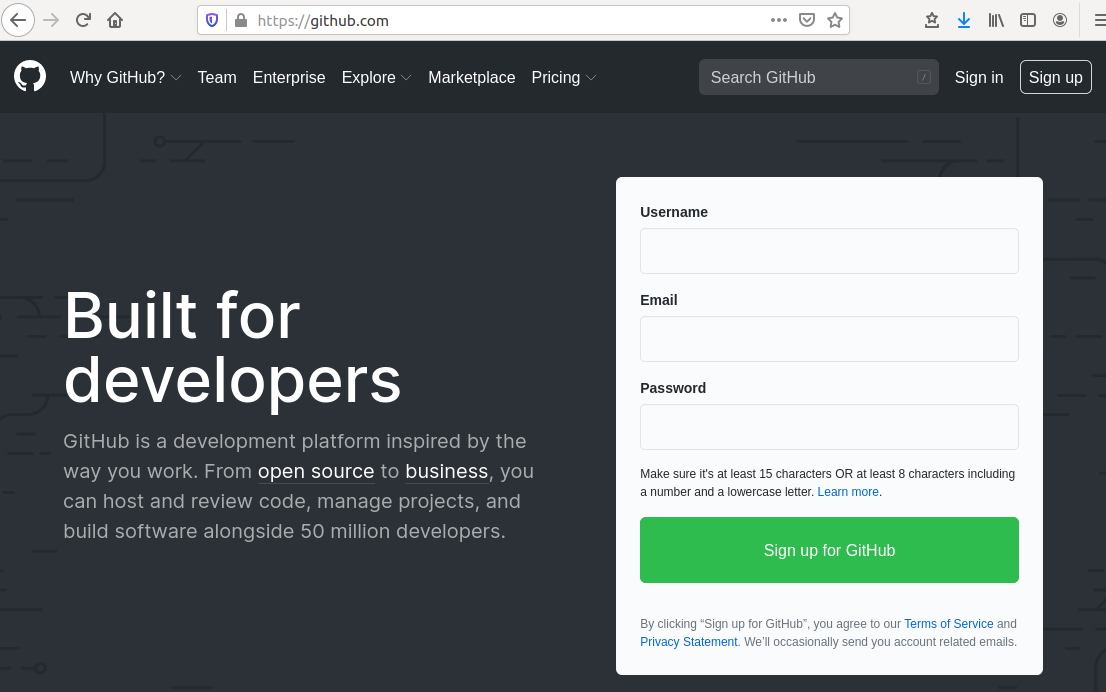
\includegraphics[height=6.4cm]{05_history/Images/FAIR_github_account.png}
\end{center}
\end{exampleblock}
\end{frame}
%-------------------------------------------
\begin{frame}{\raisebox{-1ex}{\includegraphics[height=0.8cm]{shared/logo-github.png}}: fork a project}
%-------------------------------------------
\begin{exampleblock}{Objective}
For this exercise, we will replay the addition of our first name, but by using the user interface proposed by github.
\end{exampleblock}
\begin{exampleblock}{Fork in our gituhb account}
% TODO : choisir si fork Céline ou Claire ?? changer les noms du répertoire dans le texte (dias suivantes)
With a browser, go to the url of the initial project,\href{https://github.com/chernan/super-umbrella}{\textcolor{blue}{\underline{super-umbrella}}} and click to "Fork" (upper right):
\begin{center}
    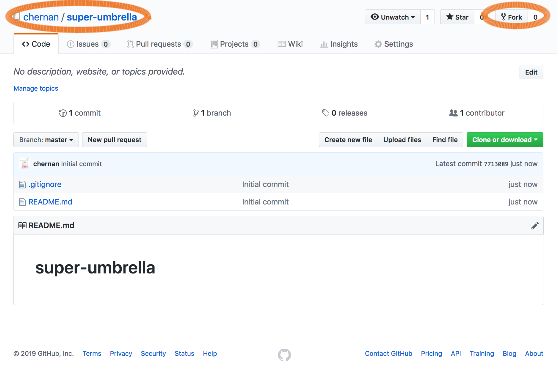
\includegraphics[height=4cm]{05_history/Images/FAIR_githubTP_fork.png}
\end{center}
\end{exampleblock}
\end{frame}
%-------------------------------------------
\begin{frame}[containsverbatim]
\frametitle{\raisebox{-1ex}{\includegraphics[height=0.8cm]{shared/logo-github.png}}: the forked repository}
%-------------------------------------------
\begin{exampleblock}{Result:}
You can see the result in your Github Overview: you have a new repository, named \verb|FAIR_bioinfo_github| and entitled "forked from chernan\verb|/|super-umbrella".
\end{exampleblock}
\begin{exampleblock}{result of the fork chernan, super-umbrella project:}
    \begin{center}
    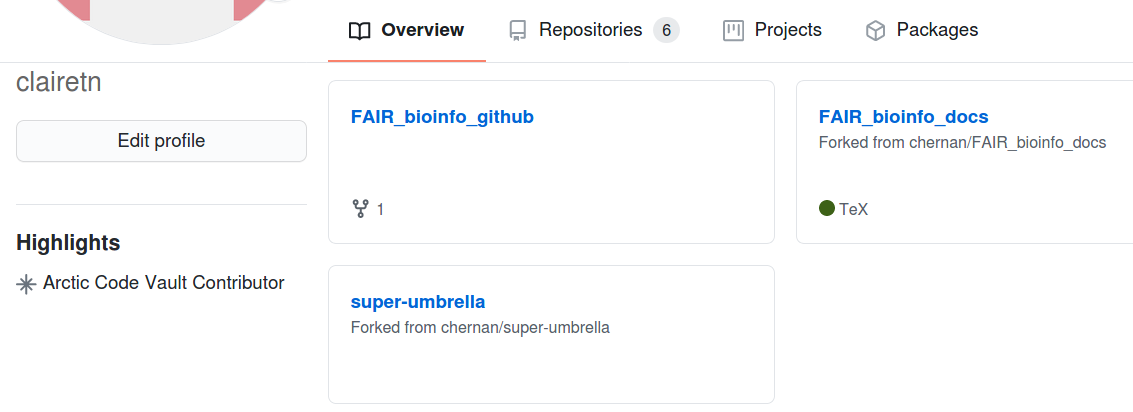
\includegraphics[height=4cm]{05_history/Images/FAIR_githubTP_forkOk.png}
    \end{center}
\end{exampleblock}
\end{frame}
%-------------------------------------------
\begin{frame}{\raisebox{-1ex}{\includegraphics[height=0.8cm]{shared/logo-github.png}} interface}
%-------------------------------------------
\begin{exampleblock}{Tabs}
8 Tabs offered by GitHub for each repository: \\
Code, Pull Requests, Actions, Projects, Wiki, Security, Insights, Settings.\\
Mainly focus on 3 of them:
\end{exampleblock}
\begin{columns}
\begin{column}{0.38\textwidth}
\begin{exampleblock}{Code}
\begin{center}
    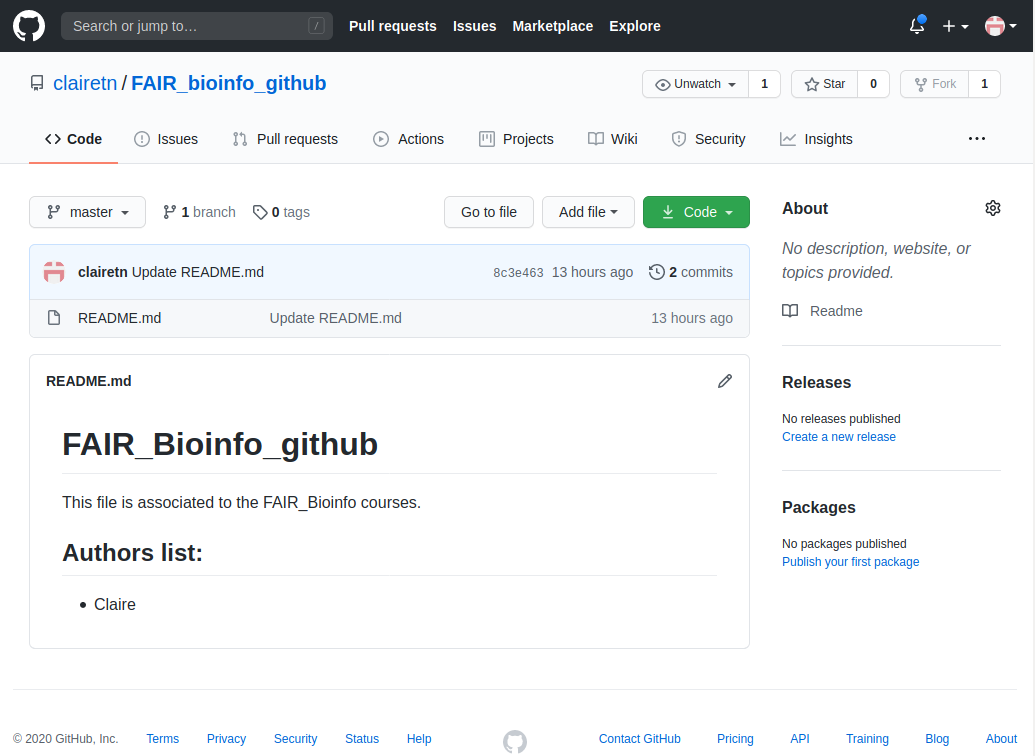
\includegraphics[height=2.8cm]{05_history/Images/FAIR_github_CodeTab.png}
\end{center}
\end{exampleblock}
\end{column}
\begin{column}{0.38\textwidth}
\begin{exampleblock}{Pull Requests}
\begin{center}
    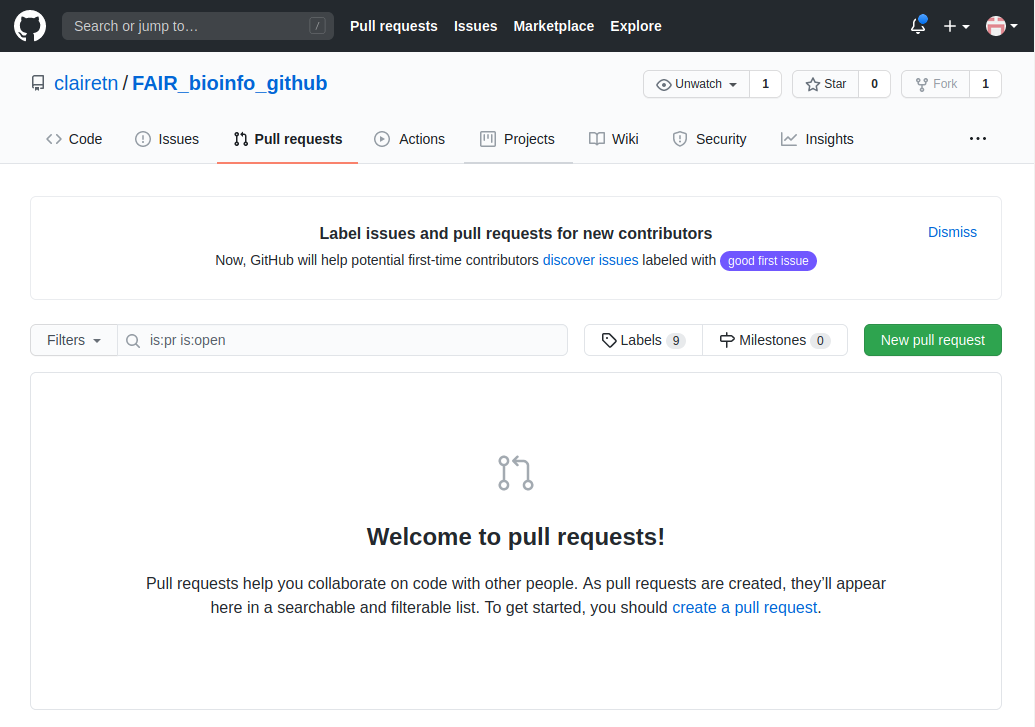
\includegraphics[height=2.7cm]{05_history/Images/FAIR_github_PullTab.png}
\end{center}
\end{exampleblock}
\end{column}
\begin{column}{0.2\textwidth}
\begin{exampleblock}{Wiki}
\begin{center}
    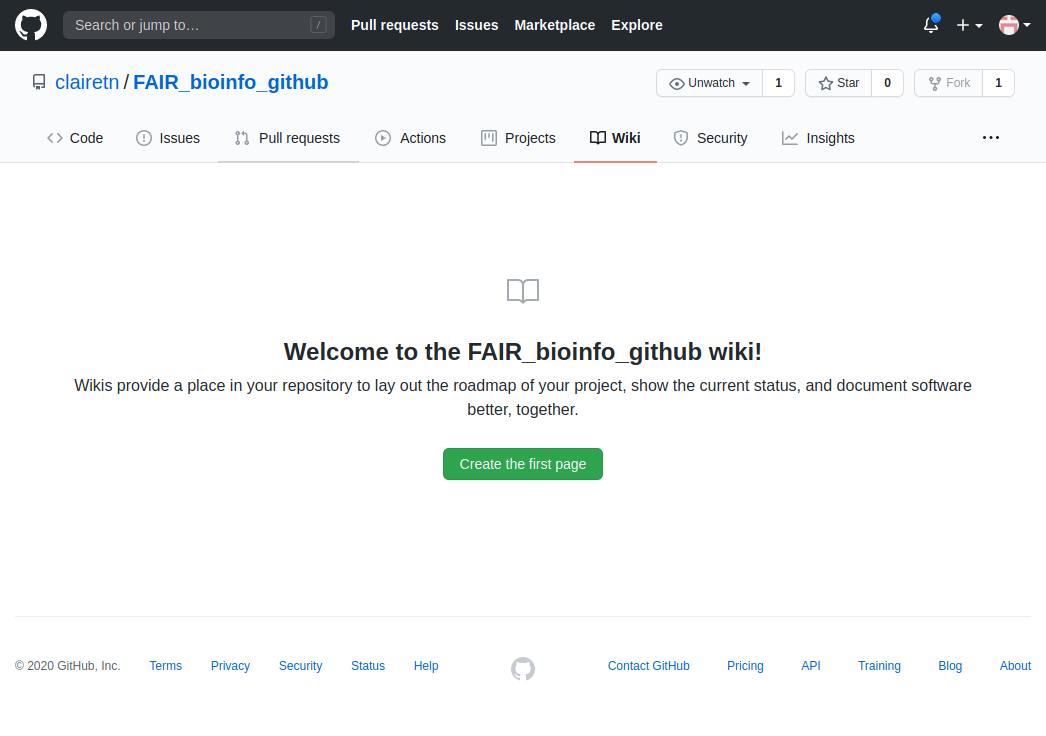
\includegraphics[height=2cm]{05_history/Images/FAIR_github_WikiTab.png}
\end{center}
\end{exampleblock}
\end{column}
\end{columns}
\end{frame}
%-------------------------------------------
\begin{frame}{\raisebox{-1ex}{\includegraphics[height=0.8cm]{shared/logo-github.png}} }
%-------------------------------------------
\begin{columns}
\begin{column}{0.49\textwidth}
\begin{exampleblock}{Previous exercises with git}
\begin{itemize}
    \item copy a github repo. (git clone)
    \item go to the local repo. (cd)
    \item create branch (git branch)
    \item go to branch (git checkout)
    \item make change (edit file)
    \item stage change (add)
    \item version change (commit)
    \item go to master (git checkout)
    \item merge branch (git merge)
    \item delete branch (git branch -d)
\end{itemize}
\end{exampleblock}
\end{column}
\begin{column}{0.49\textwidth}
\begin{exampleblock}{Next steps with github GUI:}
\begin{enumerate}
    \item fork a github repo. (just done)
    \item create branch 
    \item make change (edit file)
    \item version change (commit)
    \item compare branch to master
    \item merge branch 
    \item ask for merging (Pull Request)
    \item delete branch
\end{enumerate}
\end{exampleblock}
\end{column}
\end{columns}
\end{frame}
%--------------------------------------------


% captures d'écran différentes selon le dépôt de départ:

%%-------------------------------------------
\begin{frame}{\raisebox{-1ex}{\includegraphics[height=0.8cm]{shared/logo-github.png}} }
%-------------------------------------------
\begin{columns}
\begin{column}{0.5\textwidth}
\begin{exampleblock}{2: create branch1}
    \begin{center}
    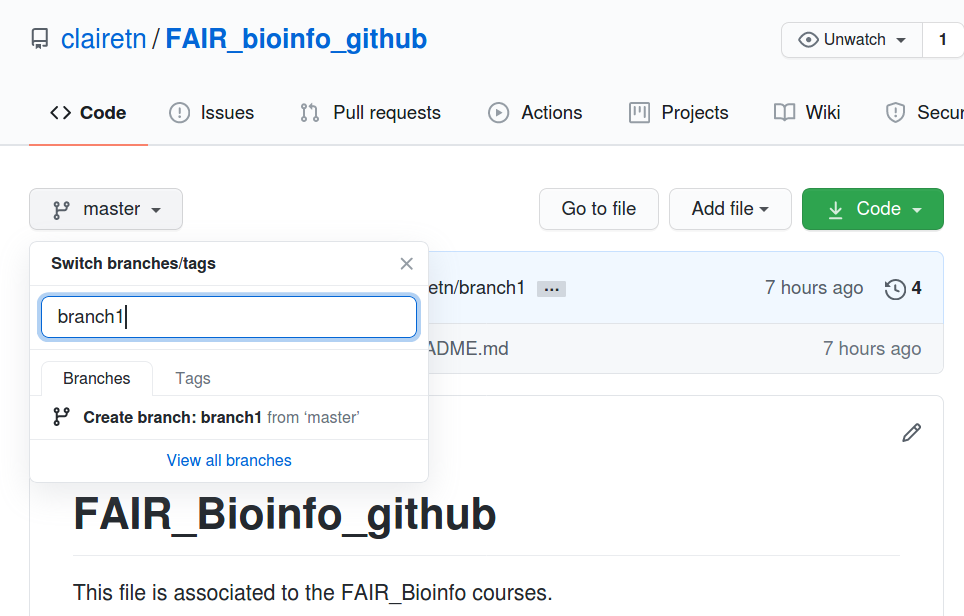
\includegraphics[height=3.8cm]{05_history/Images/FAIR_github_branch1.png}
    \end{center}
\end{exampleblock}
\end{column}
\begin{column}{0.46\textwidth}
\begin{exampleblock}{branch1 created}
    \begin{center}
    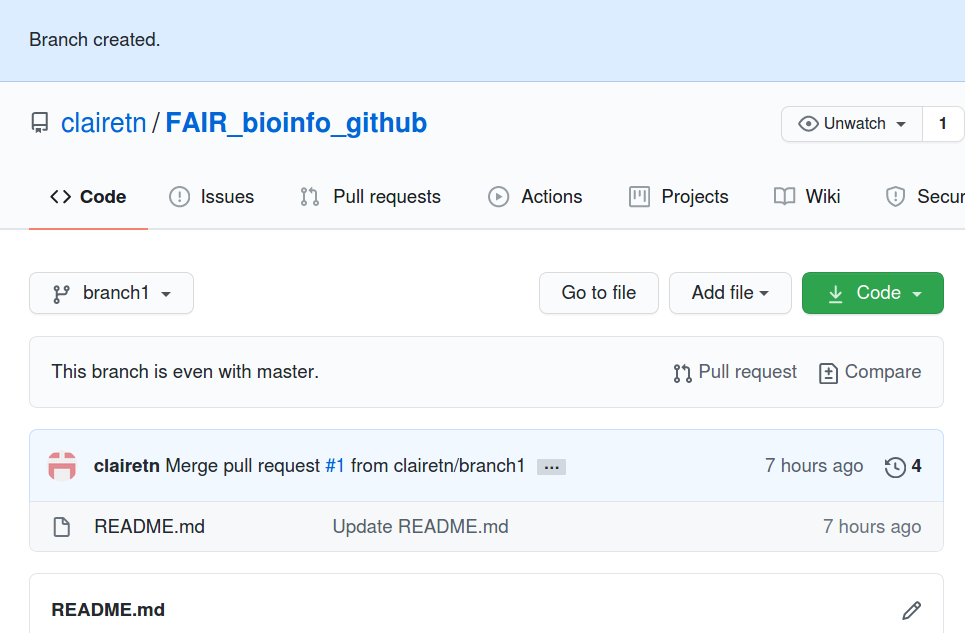
\includegraphics[height=3.6cm]{05_history/Images/FAIR_github_branch1ok.png}
    \end{center}
\end{exampleblock}
\end{column}
\end{columns}
\end{frame}
%-------------------------------------------
\begin{frame}{\raisebox{-1ex}{\includegraphics[height=0.8cm]{shared/logo-github.png}} }
%-------------------------------------------
\begin{columns}
\begin{column}{0.48\textwidth}
\begin{exampleblock}{3: make change (Edit, click pen)}
    \begin{center}
    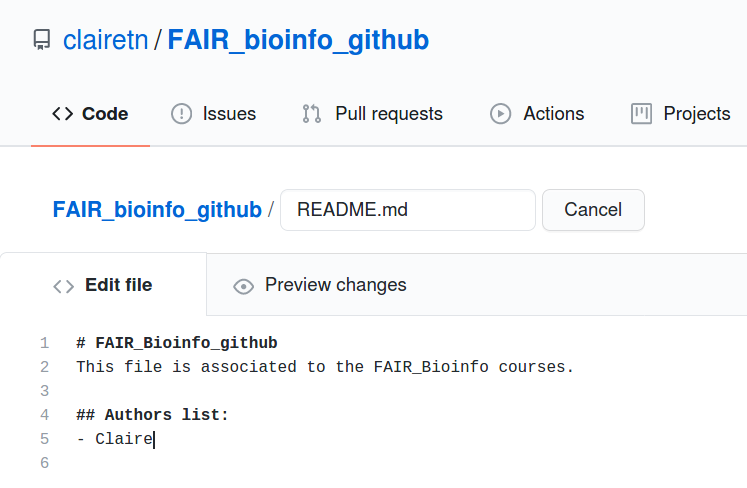
\includegraphics[height=3.6cm]{05_history/Images/FAIR_github_EditFile.png}
    \end{center}
\end{exampleblock}
\end{column}
\begin{column}{0.48\textwidth}
\begin{exampleblock}{4: commit (bottom page)}
    \begin{center}
    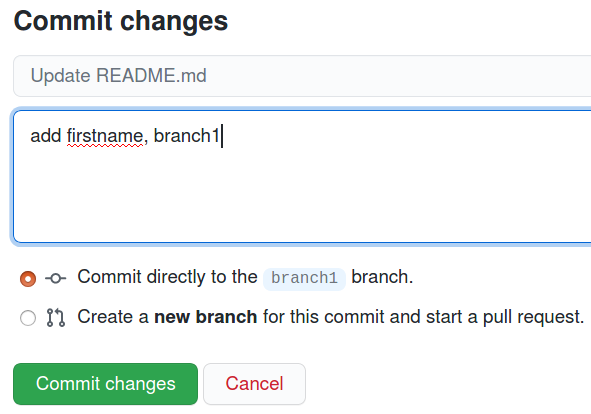
\includegraphics[height=3.6cm]{05_history/Images/FAIR_github_Commit.png}
    \end{center}
\end{exampleblock}
% TODO ajouter une flèche orange vers le bas pour indiquer que la dias suivante en en bas de la page 
\end{column}
\end{columns}
\end{frame}
%-------------------------------------------
\begin{frame}{\raisebox{-1ex}{\includegraphics[height=0.8cm]{shared/logo-github.png}} }
%-------------------------------------------
\begin{columns}
\begin{column}{0.48\textwidth}
\begin{exampleblock}{5: Compare}
    \begin{center}
    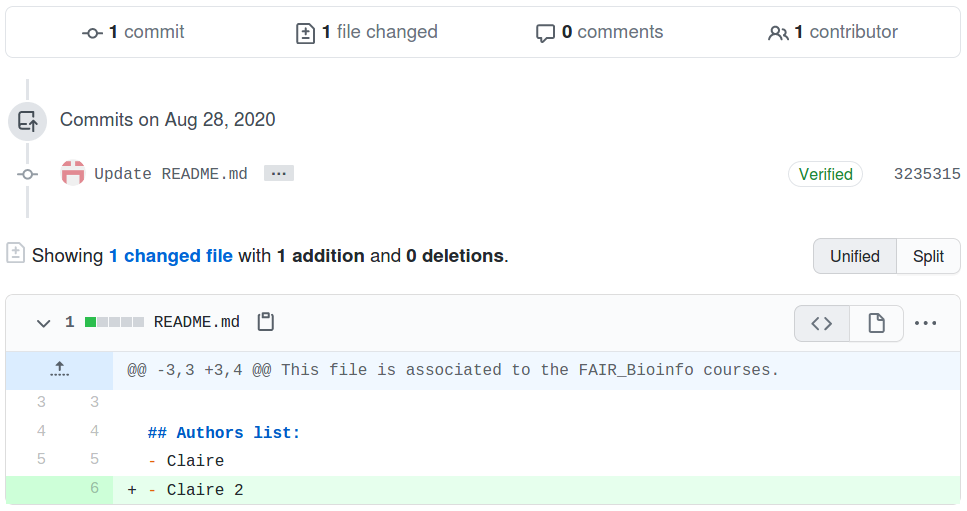
\includegraphics[height=3cm]{05_history/Images/FAIR_github_compareBranch1.png}
    \end{center}
\end{exampleblock}
 take some time to appear ...
\end{column}
\begin{column}{0.48\textwidth}
\begin{exampleblock}{6: Pull request commit}
    \begin{center}
    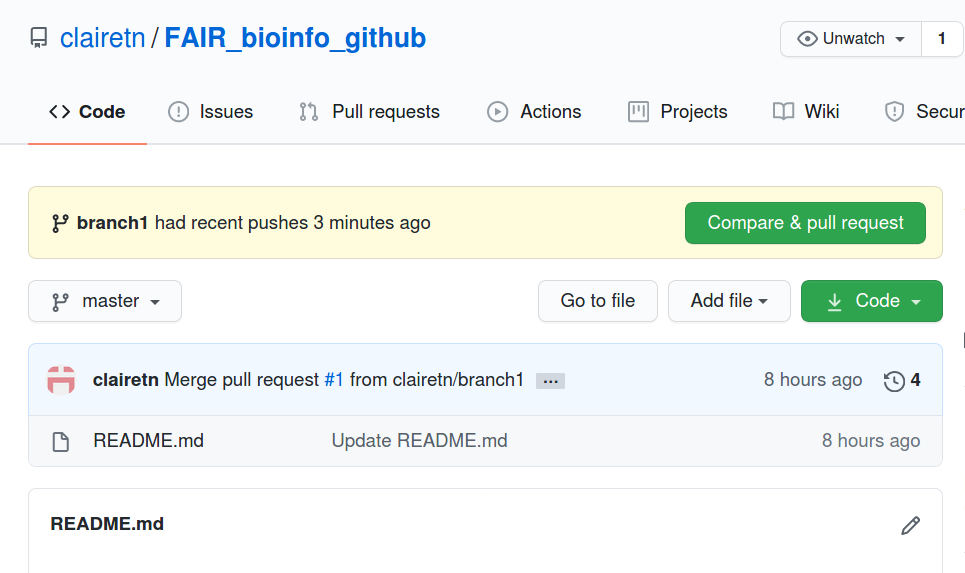
\includegraphics[height=2.8cm]{05_history/Images/FAIR_github_comparePull.png}
    \end{center}
\end{exampleblock}
\end{column}
\end{columns}
\end{frame}
%-------------------------------------------
\begin{frame}{\raisebox{-1ex}{\includegraphics[height=0.8cm]{shared/logo-github.png}} }
%-------------------------------------------
\begin{columns}
\begin{column}{0.48\textwidth}
\begin{exampleblock}{7: Merge branch1}
    \begin{center}
    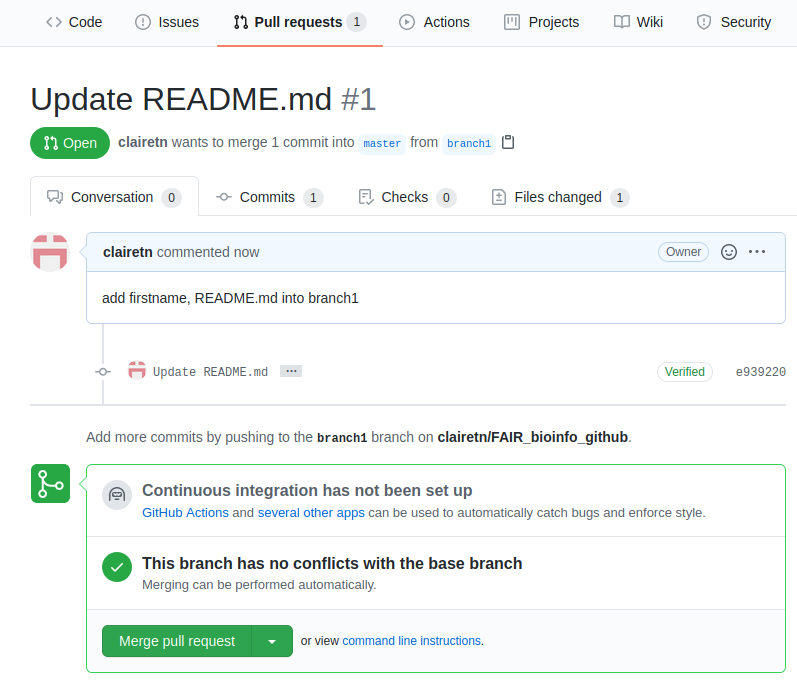
\includegraphics[height=4.5cm]{05_history/Images/FAIR_github_PullRequestBranch1.png}
    \end{center}
\end{exampleblock}
\end{column}
\begin{column}{0.48\textwidth}
\begin{exampleblock}{8: Pull request merge}
    \begin{center}
    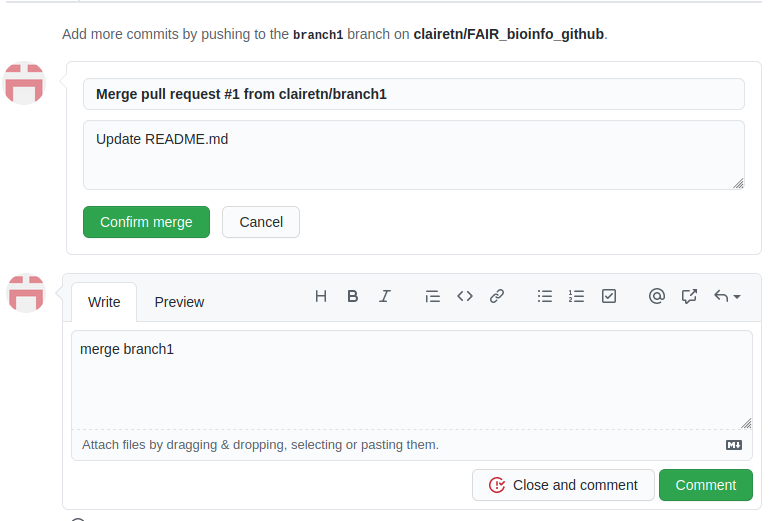
\includegraphics[height=3.5cm]{05_history/Images/FAIR_github_MergeBranch1.png}
    \end{center}
\end{exampleblock}
\end{column}
\end{columns}
\end{frame}
%-------------------------------------------
\begin{frame}{\raisebox{-1ex}{\includegraphics[height=0.8cm]{shared/logo-github.png}} }
%-------------------------------------------
\begin{columns}
\begin{column}{0.49\textwidth}
\begin{exampleblock}{Merge success}
    \begin{center}
    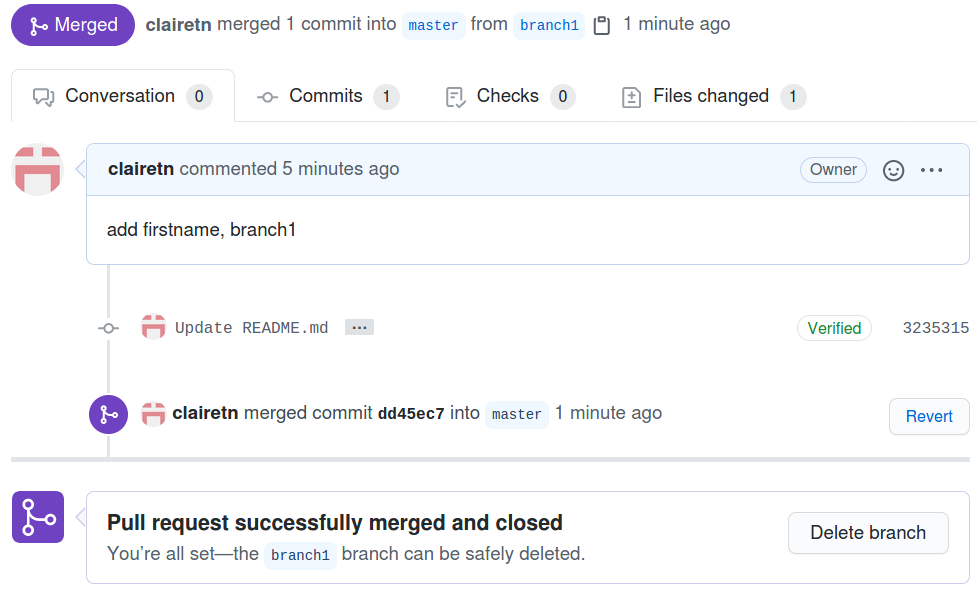
\includegraphics[height=3.5cm]{05_history/Images/FAIR_github_MergeSucceed.png}
    \end{center}
\end{exampleblock}
\end{column}
\begin{column}{0.49\textwidth}
\begin{exampleblock}{9: Delete branch1}
    \begin{center}
    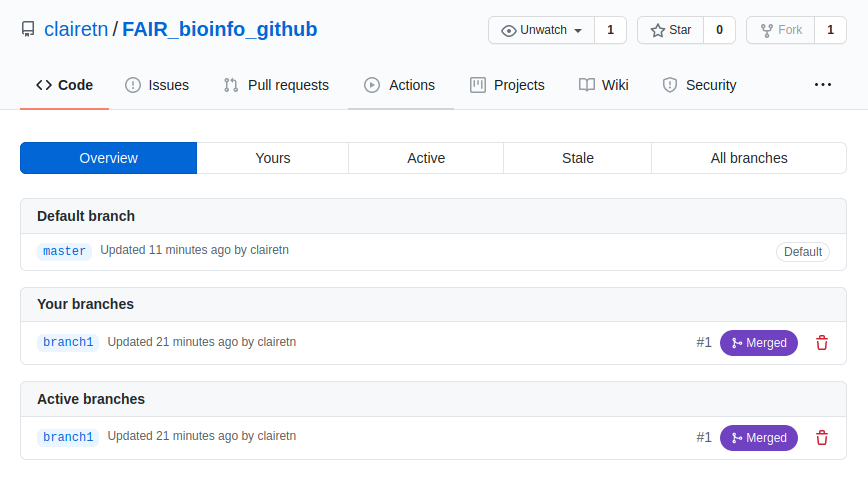
\includegraphics[height=3.4cm]{05_history/Images/FAIR_github_DeleteBranch1.png}
    \end{center}
\end{exampleblock}
\end{column}
\end{columns}
\end{frame}

%-------------------------------------------
\begin{frame}{\raisebox{-1ex}{\includegraphics[height=0.8cm]{shared/logo-github.png}} }
%-------------------------------------------
\begin{exampleblock}{1: fork chernan, super-umbrella, see the README.md file:}
    \begin{center}
    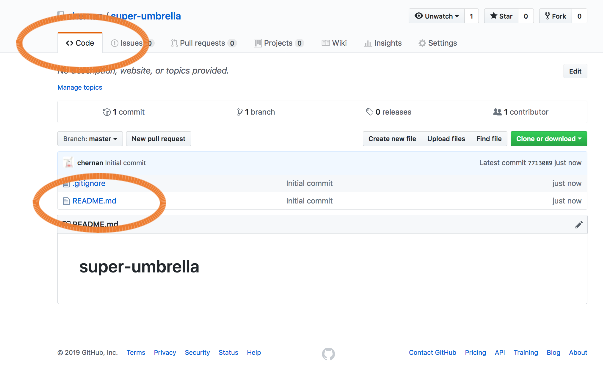
\includegraphics[height=6cm]{05_history/Images/FAIR_githubTP_readme.png}
    \end{center}
\end{exampleblock}
\end{frame}
%-------------------------------------------
\begin{frame}{\raisebox{-1ex}{\includegraphics[height=0.8cm]{shared/logo-github.png}} }
%-------------------------------------------
\begin{exampleblock}{2: create a new branch, named "devel-your-name"}
    \begin{center}
    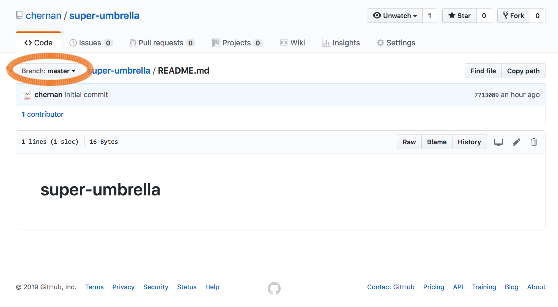
\includegraphics[height=6.5cm]{05_history/Images/FAIR_githubTP_develBranch.png}
    \end{center}
\end{exampleblock}
\end{frame}

%-------------------------------------------
\begin{frame}{\raisebox{-1ex}{\includegraphics[height=0.8cm]{shared/logo-github.png}} }
%-------------------------------------------
\begin{exampleblock}{3: edit README.md to make change}
    \begin{center}
    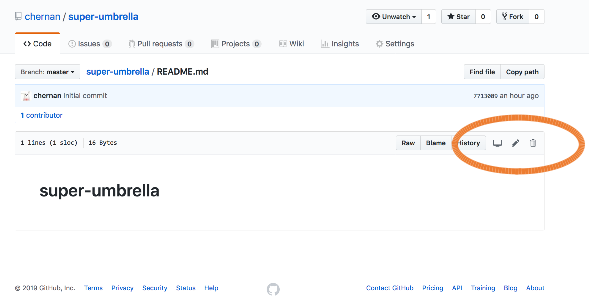
\includegraphics[height=6cm]{05_history/Images/FAIR_githubTP_edit.png}
    \end{center}
\end{exampleblock}
\end{frame}
%-------------------------------------------
\begin{frame}{\raisebox{-1ex}{\includegraphics[height=0.8cm]{shared/logo-github.png}} }
%-------------------------------------------
\begin{exampleblock}{3: make change}
    \begin{center}
    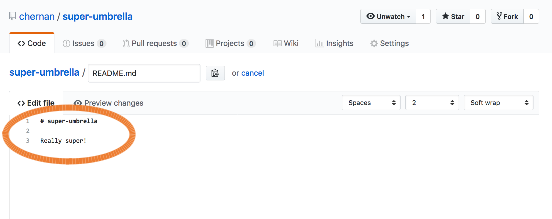
\includegraphics[height=4.5cm]{05_history/Images/FAIR_githubTP_editing.png}
    \end{center}
\end{exampleblock}
\end{frame}
%-------------------------------------------
\begin{frame}{\raisebox{-1ex}{\includegraphics[height=0.8cm]{shared/logo-github.png}} }
%-------------------------------------------
\begin{exampleblock}{4: commit}
    \begin{center}
    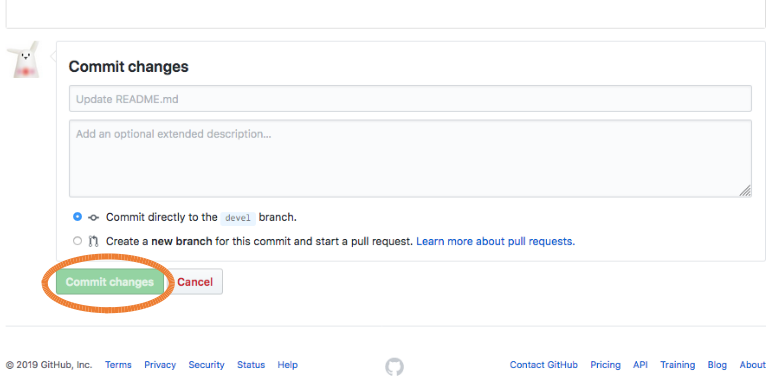
\includegraphics[height=6cm]{05_history/Images/FAIR_githubTP_commit.png}
    \end{center}
\end{exampleblock}
\end{frame}
%-------------------------------------------
\begin{frame}{\raisebox{-1ex}{\includegraphics[height=0.8cm]{shared/logo-github.png}} }
%-------------------------------------------
\begin{exampleblock}{4: commit and pull request}
    \begin{center}
    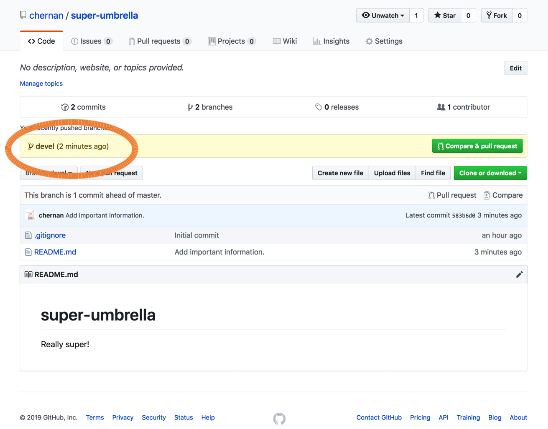
\includegraphics[height=6cm]{05_history/Images/FAIR_githubTP_commitOk.png}
    \end{center}
\end{exampleblock}
\end{frame}
%-------------------------------------------
\begin{frame}{\raisebox{-1ex}{\includegraphics[height=0.8cm]{shared/logo-github.png}} }
%-------------------------------------------
\begin{exampleblock}{5: pull request, compare}
    \begin{center}
    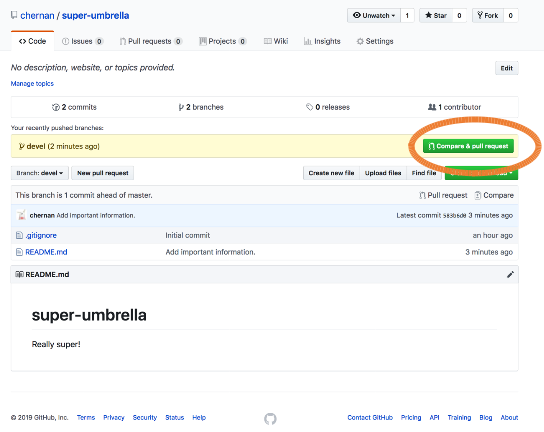
\includegraphics[height=6cm]{05_history/Images/FAIR_githubTP_comparePR.png}
    \end{center}
\end{exampleblock}
\end{frame}
%-------------------------------------------
\begin{frame}{\raisebox{-1ex}{\includegraphics[height=0.8cm]{shared/logo-github.png}} }
%-------------------------------------------
\begin{exampleblock}{5: pull request, able to merge}
    \begin{center}
    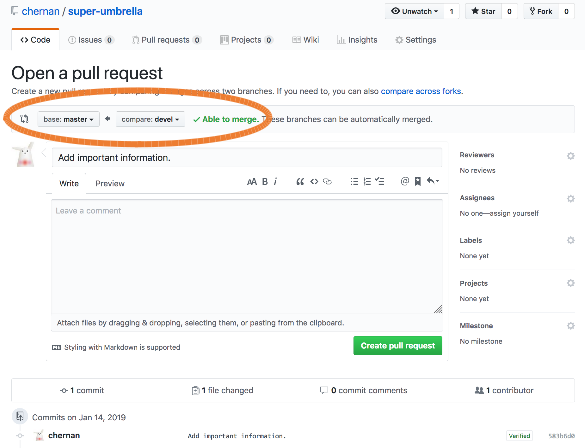
\includegraphics[height=6cm]{05_history/Images/FAIR_githubTP_mergeEnable.png}
    \end{center}
\end{exampleblock}
\end{frame}
%-------------------------------------------
\begin{frame}{\raisebox{-1ex}{\includegraphics[height=0.8cm]{shared/logo-github.png}} }
%-------------------------------------------
\begin{exampleblock}{5: merge and pull request}
    \begin{center}
    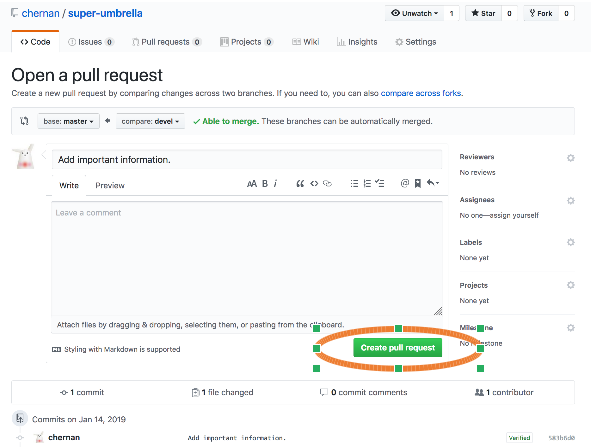
\includegraphics[height=6cm]{05_history/Images/FAIR_githubTP_openMergePR.png}
    \end{center}
\end{exampleblock}
\end{frame}
%-------------------------------------------
\begin{frame}{\raisebox{-1ex}{\includegraphics[height=0.8cm]{shared/logo-github.png}} }
%-------------------------------------------
\begin{exampleblock}{5: merge and Pull request}
    \begin{center}
    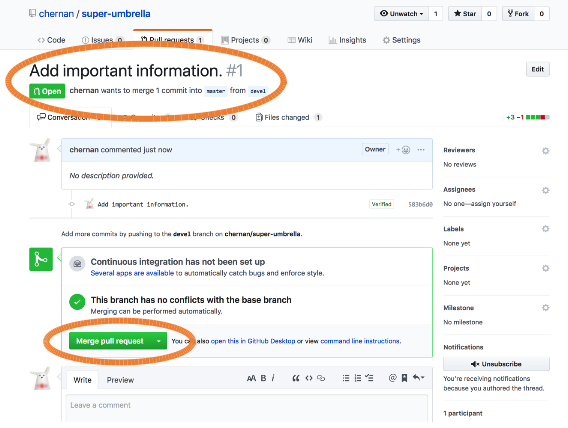
\includegraphics[height=7cm]{05_history/Images/FAIR_githubTP_mergePR.png}
    \end{center}
\end{exampleblock}
\end{frame}
%-------------------------------------------
\begin{frame}{\raisebox{-1ex}{\includegraphics[height=0.8cm]{shared/logo-github.png}} }
%-------------------------------------------
\begin{exampleblock}{5: merge and Pull request}
    \begin{center}
    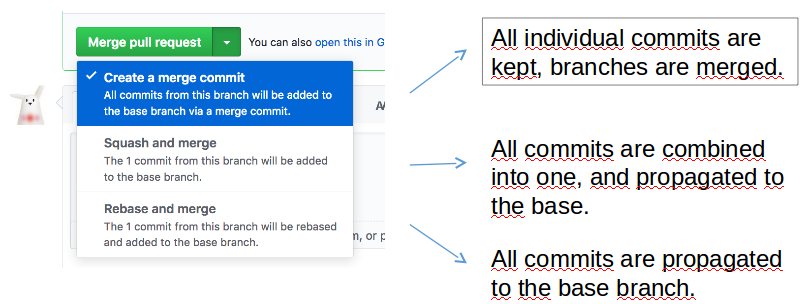
\includegraphics[height=4.5cm]{05_history/Images/FAIR_githubTP_mergeConfig.png}
    \end{center}
\end{exampleblock}
\end{frame}
%-------------------------------------------
\begin{frame}{\raisebox{-1ex}{\includegraphics[height=0.8cm]{shared/logo-github.png}} }
%-------------------------------------------
\begin{exampleblock}{6: merge}
    \begin{center}
    \includegraphics[height=7cm]{05_history/Images/FAIR_githubTP_confirmMerge.png}
    \end{center}
\end{exampleblock}
\end{frame}
%-------------------------------------------
\begin{frame}{\raisebox{-1ex}{\includegraphics[height=0.8cm]{shared/logo-github.png}} }
%-------------------------------------------
\begin{exampleblock}{7: the merge delete the branch}
    \begin{center}
    \includegraphics[height=6cm]{05_history/Images/FAIR_githubTP_mergeOk.png}
    \end{center}
\end{exampleblock}
\end{frame}
%-------------------------------------------
\begin{frame}{\raisebox{-1ex}{\includegraphics[height=0.8cm]{shared/logo-github.png}} }
%-------------------------------------------
\begin{exampleblock}{See version network, Insights tab}
    \begin{center}
    \includegraphics[height=6cm]{05_history/Images/FAIR_githubTP_insights.png}
    \end{center}
\end{exampleblock}
\end{frame}



%-------------------------------------------
\begin{frame}{\raisebox{-1ex}{\includegraphics[height=0.8cm]{shared/logo-github.png}} Conclusion}
%-------------------------------------------
\begin{exampleblock}{GitHub GUI}
\begin{itemize}
    \item With this exercise, we modified a file in a directory of our own GitHub account. 
    \item BUT: reserve this click button mode only for minor modifications (relies on a stable and smooth network connection!)
    \item Also, we collaborated only with ourselves
    \item In the next exercise, we will do this task again with a "git command line" mode and by collaborating all together.
\end{itemize}
\end{exampleblock}
\end{frame}

